\documentclass[12pt]{article}%%contributed-IMS
\usepackage{amsthm,amsmath,amsfonts,amssymb,natbib}
\usepackage{graphicx}
\pagestyle{empty}

%\setlength{\textwidth}{7in}
%\setlength{\oddsidemargin}{-.25in}
%\setlength{\evensidemargin}{-.25in}


\newtheorem{lem}{Lemma}

\title{TBD}
\author{Nam H. Lee \& c}
\begin{document}
\maketitle

\section{Overview}
For each (undirected) pair $ij$ of $n$ vertices and each $t \in [0,1]$,
we let $N_{ij}(t)$ be the number of (undirected) communication events between vertex $i$ and vertex $j$, where each event is marked with one of the communication content topic classes $\{1,2\}$. 
Let, for each $t \in [0,1]$,
$$
\mathcal D(t) = \{ (\tau_\ell, ij_{\ell}, k_{\ell}) : \ell=1,\ldots, N(t) \},
$$ 
where $N(t) = \sum_{i<j} N_{ij}(t)$ and for simplicity, let 
$$
\mathcal D = \mathcal D(1).
$$ 

In this paper, we consider a problem of classifying the $n$ vertices into two groups after seeing $\mathcal D$, where the members of each class have the similar degrees of interests in topics from two content topic classes.  For this, we propose a classification algorithm derived from an EM-based paramter estimation procedure. 

To formulate our EM-based algorithm, we introduce a model for $\mathcal D$ through a data augmentation principle.  The hidden variables augmenting the data are the collection of random variables $\{\Lambda_{i,k}(t)\}$, where $\Lambda_{i,k}(t)$ is the degree of vertex $i$'s interest in topics from content topic class $k$ at time $t$. We assume that each $\Lambda_{i,k}(t)$ is a strictly positive random variable such that for some fixed constant $\lambda_i \in (0,\infty)$,
\begin{eqnarray}
\lambda_i = \Lambda_{i,1}(t) + \Lambda_{i,2}(t).
\end{eqnarray}
Our model, yielding the observation $\mathcal D$, is then to be a doubly stochastic marked Poisson process whose latent intensity process is specified by the $n\times 2$ random matrix
\begin{eqnarray}
\Lambda(t) = (\Lambda_{i,k}(t); i=1,\ldots,n, k=1,2).
\end{eqnarray}
For convenience, we denote the $i$-th row of $\Lambda(t)$ by $\Lambda_i(t)$. 

To demonstrate the peformance of our classification algorithm, we will also consider a so-called vertex nomination problem, in which the memembers of a particular class is already known and the objective is then to decide whether or not the class is to be expanded further and if to be expanded, which (single) vertex is to be included next. A solution to the vertex nomination problem is likely to be useful if some other information other than $\mathcal D$ is available.  On the other hand, we will also denomstrate the peformance of our classification algorithm when the only available information is $\mathcal D$ and the vertex nomination is then interpreted as a two-pass procedure.  

\section{Single-period model}
For each vertex $i$ and time $t\in[0,1]$, let 
\begin{eqnarray}
X_i(t) = (X_{i,1}(t), X_{i,2}(t)),
\end{eqnarray}
where
\begin{eqnarray}
X_{i,k}(t) = \frac{\Lambda_{i,k}(t)}{\Lambda_i(t)},
\end{eqnarray}
and note that each $X_i(t)$ is a probability vector. 
For each (undirected) pair $ij$, we assume that 
the process $N_{ij} = (N_{ij}(t):t\in[0,1])$ is   
a doubly stocastic Poisson process that whose intensity process is  
\begin{eqnarray}
\Lambda_{ij}(t) = \lambda_i \lambda_j (X_{i,1}(t)X_{j,1}(t) + X_{i,2}(t)X_{j,2}(t)).
\end{eqnarray}
A particularly useful chracterization is to describe each $N_{ij}$ as a process obtained 
by thinning a homogeneous Poisson process $C_{ij}$ whose constant intensity is $\lambda_i \lambda_j$.  
This affords an interpretation that each $t$ such that $C_{ij}(t) = C_{ij}(t-) +1$ 
is a potential communication opportunity between vertex $i$ and vertex $j$, 
and at each such $t$, depending on values of $X_i(t)$ and $X_j(t)$, 
the opportunity may or may not give rise to an actual communication event, i.e.\ $t$ such that $N_{ij}(t) = N_{ij}(t-) +1$. To be more precise, it is our assumption that given the filtration 
$$
\mathcal F_{ij}^\Lambda(t) = \sigma(\Lambda_i(s), \Lambda_j(t): s \le t), 
$$
if $C_{ij}(t) = C_{ij}(t-)+1$, then
$N_{ij}(t) = N_{ij}(t-) + 1$ with probability $\Lambda_{ij}(t)$ and the topic mark is of content class $k$ with probaiblity 
$$
\frac{X_{i,k}(t)X_{j,k}(t)}{X_{i,1}(t)X_{j,1}(t) + X_{i,2}(t)X_{j,2}(t)}
=
\frac{\Lambda_{i,k}(t)\Lambda_{j,k}(t)}{\Lambda_{i,1}(t)\Lambda_{j,1}(t) + \Lambda_{i,2}(t)\Lambda_{j,2}(t)}.
$$
Now, we fix a stationary diffusion process $Y_i=(Y_i(t):t\in [0,1])$ such that  
\begin{eqnarray}
dY_i(t) = \mu(Y_t(t)) dt + \sigma_i(Y_i(t)) dB_i(t),
\end{eqnarray}
where each $\mu_i$ and $\sigma_i$ are twice continuously and boundedly differentiable functions, and $B_1,\ldots,B_n$ are independent standard Brownian motions.
In fact, in this paper, for concreteness, we assume that 
\begin{eqnarray}
dY_i(t) = \beta_i (\mu_i - Y_i(t)) dt + \sigma_i dB_i(t),
\end{eqnarray}
for some fixed constants $\mu_1,\ldots, \mu_n \in \mathbb R$, and $\sigma_1 = \ldots = \sigma_n \in (0,\infty)$ and $\beta_1 = \ldots = \beta_n \in (0,\infty)$. 
Then, we assume that 
\begin{eqnarray}
X_{i,1}(t) = \frac{\exp(-Y_i(t)}{1+\exp(-Y_i(t))}.
\end{eqnarray}
While we could also take $\sigma_1,\ldots,\sigma_n$ and $\beta_1,\ldots, \beta_n$ to be parameters, 
but for our vertex nomination problem or more generally classification problem, 
these potential paramters are (perhaps) nuisance parameters (?).  
In our algorithm, we propose to fix the nusiance parameters before proceding to a classification/vertex notimation task.
Finally, for future reference, we let
$$
\psi = (\mu_1,\ldots, \mu_n,\lambda_1,\ldots,\lambda_n).
$$

\section{Greedy algorithm for iterative vertex nomination}
 
Our main result of this paper concerns an algorithm 
for correctly assigning each vertex into one of two classes, where witnin each group, all the members  
have the same parameter i.e.\ if vertex $i$ and vertex $j$ are in the same
class, then $\psi_i = \psi_j$.  
In this section, we provide a greedy algorithm for arriving at a partition 
of the vertex set which is likely to be the true partition of 
the vertex set that  have produced the data $\mathcal D$.

For the initial step $q=1$, suppose that we have 
an arbitrary partition $(C_1(1), C_2(1))$ of $\{1,\ldots, n\}$. 
Let $\psi^1$ be the output of our EM algorithm, where we assume that within each group,
all vertice have the same paramter.  Then, for each pair $i, j \in C_k(1)$, $\psi_i^1 = \psi_j^1$.  
Let
\begin{eqnarray}
Q(1) : = \mathbf E_{\psi(1)}\left[\log(f(\mathcal D, Y;\psi^1))\right],
\end{eqnarray}
where $f(;\psi)$ denote the likelikehood function of observing $\mathcal D$ and $Y$ with the given parameter $\psi$ (see the next section for more details about this). 
Next, for the $(r+1)$-st iteration, suppose that we have a partition $(C_1(r), C_2(r))$ from the $r$-th iteration. 
If $C_2(r) = \varnothing$, then our partitioning algorithm terminates, yielding the $r$-th partition 
$(C_1(r), C_2(r))$ as the final output.  So, we assume that $C_2(r)\neq \varnothing$.  Then, for some $\ell > 0$ and $m > 0$ with $\ell + m = n$, we have 
\begin{eqnarray}
&C_1(r) = \{u_1,\ldots, u_\ell\},\\
&C_2(r) = \{v_1,\ldots, v_m\}.
\end{eqnarray} 
For each $i \in C_2(r)$, let 
\begin{eqnarray}
&C_1^{i}(r) = C_1(r) \cup \{i\}, \\
&C_2^{i}(r) = C_2(r) \setminus \{i\}.
\end{eqnarray}
Now, for each $i$, let $\psi^{i,r}$ be the EM estimate of $\psi$ with the partition $(C_1^{i}(r), C_2^{i}(r))$, and let 
\begin{eqnarray}
Q^{i}(r) = \mathbf E_{\psi^{i,r}}\left[\log(f(\mathcal D,Y;\psi^{i,r}))\right].
\end{eqnarray}
If for all $i \in C_2(r)$, $Q^{i}(r) \le Q(r)$, then the algorithm terminates, yielding 
$(C_1(r), C_2(r))$ as the final partitioning.  Otherwise, we set 
\begin{eqnarray}
i^* = \arg\max_{i \in C_2(r)} Q^{i}(r),
\end{eqnarray}
and let 
\begin{eqnarray}
&C_1(r+1) = C_1(r) \cup \{i^*\},\\
&C_2(r+1) = C_2(r) \setminus \{i^*\}.
\end{eqnarray}



\section{Estimation by EM procedure}
\subsection{Overview}
Let
\begin{enumerate}
\item[(i)] $M_{ij}$ is the (total) number of messages between vertex $i$ and vertex $j$,
\item[(2)] $\tau_{ij}(\ell)$ is the time at which occurred the $\ell$-th communication event  between vertex $i$ and vertex $j$.
\end{enumerate}
In the expectation stage of our EM algorithm, for each $\psi$, we compute the expected value of the following random variable:
\begin{eqnarray}
\prod_{i<j} f_{ij}(\mathcal D(ij);X_i^r,X_j^r,\psi) \prod_{i=1}^n f_{i}(Y_i^r;\psi),
\end{eqnarray}
where 
\begin{enumerate}
\item[(i)] $Y_i^r$ is a diffusion process whose distribution is a conditional distribution of $Y_i$ given the observation $\mathcal D$ with the unconditional distribution of $Y_i$ for the $r$-th estimated parameter $\psi^r$,
\item[(ii)] $f_{i}(\cdot;\psi)$ is the likelihood of the $i$-th vertex 
process' sample path $Y_i$ with the parameter $\psi$,
\item[(iii)] $f_{ij}(\cdot;X_i^r,X_j^r,\psi)$ specifies the conditional likelidhood given $X_1^r,\ldots,X_n^r$ of 
observing message at time 
$$
\tau_{ij}(1),\ldots, \tau_{ij}(M_{ij}),
$$
repsectively, about topic 
$$
\kappa_{ij}(1),\ldots, \kappa_{ij}(M_{ij}).
$$
\end{enumerate}

   
Note that conditioning on the path of $Y_i$ and $Y_j$ (but not on $\mathcal D)$, and given the value of $\psi$, the value of $f_{ij}(\cdot;X_i,X_j,\psi)$ can be seen to be
\begin{eqnarray}\label{formula2010.12.19.12.31.pm}
\prod_{i<j} \left(\prod_{\ell=1}^{M_{ij}} \Lambda_{i,\kappa_{ij}(\ell)}(\tau_{ij}(\ell))\Lambda_{j,\kappa_{ij}(\ell)}(\tau_{ij}(\ell))\right) \exp\left(-\int_0^T \Lambda_{ij}(s) ds\right).
\end{eqnarray}
Next, given $\sigma_i=1$ and $\beta_i=1$ for all $i=1,\ldots, n$, 
it can be shown that
\begin{eqnarray*}
&\ &\log (f_i(Y_{i}^r(t);\psi))\\
&= & \mu_i (Y_{i}^r(1) - Y_{i}^r(0)) - \frac{1}{2} ((Y_{i}^r(1))^2 - (Y_i^r(0))^2) - \frac{1}{2} \int_0^1 (\mu_i-Y_{i}^r(t))^2 - 1 dt. 
\end{eqnarray*}


Now we remark here that while unconditionally, the diffusion processes $Y_1,\ldots, Y_n$ are independent, 
conditionally, $Y_1,\ldots,Y_n$ need not be independent.  
Computing the exact conditionally likelihood of $Y_i^r$ analytically is difficult if not practically impossible 
even for the relatively simple diffusion process $Y_1,\ldots,Y_n$ that we are considering in this paper. 
Because of this, our algorithm relies instead on an EM algorithm in where the expected value in the E step 
is estimated by simulation and in the M step, the maximization is done numerically.     
An except to this arises if we set the nusiance parameter $\sigma_1 = \ldots = \sigma_n = 0$.
In this case, each $Y_i^r = \mu_i$ and it is not difficult to see that the MLE of $\psi$ given $\mathcal D$ 
satisfies the following equations:
\begin{eqnarray}
\frac{1}{\lambda_i} \left(\sum_{j\neq i} M_{ij}\right)  -  \sum_{j\neq i} \lambda_j (2 X_i X_j + 1 - X_i - X_j) = 0,
\end{eqnarray}
\begin{eqnarray}
\frac{1}{X_{i,1}} \left(\sum_{j\neq i} M_{ij,1}\right)  + \frac{1}{1-X_{j,1}} \sum_{j\neq i} M_{ij,2} 
-
\lambda_i \sum_{j\neq i}  \lambda_j (2 X_{i,j} - 1) =0.
\end{eqnarray}

 

\subsection{Conditional sampling algorithms}
In the E step, one needs to know how to compute, for each $\psi$,
\begin{eqnarray}
Q_\ell(\psi) = \mathbf E_{\psi_\ell,\mathcal D}\left[ \log f_{[0,T]}(\mathcal D, X^{(\ell)};\psi)\right],
\end{eqnarray}
where the law of $X^{(\ell)}$ is the law of $X$ conditioning on the data $\mathcal D$ and the paramter $\psi_\ell$.  
The general closed-form expression of $Q(\psi)$ is difficult to obtain, 
and we develop a way to obtain a close approximation $\widehat{Q}_\ell$ of $Q$.  
To do this, we use a Monte Carlo estimate based on the rejection technique. 
 First, our simulation of each $X_i$ (uncondtionally) is achieved through discriteziation.  
For example, we can fix a small $\Delta t > 0$ and 
\begin{eqnarray}
Y_i(t+\Delta t) = Y_i(t) + \beta_i(\mu_i - Y_i(t)) \Delta t + \sigma_i  Z \Delta t,
\end{eqnarray}
where $Z$ is a standard normal random variable.  
Next, note that 
\begin{eqnarray}
f(Y\left|\mathcal D\right.;\psi) 
&\propto& f(Y,\mathcal D;\psi) \\
&=& f(\mathcal D\left|X,\psi\right.) f(Y\left|\psi\right.)\\
&=& \prod_{i<j} f_{ij}(\mathcal D(ij);X_i,X_j,\psi) \prod_{i=1}^n f_{i}(Y_i;\psi),\\
&\le & \prod_{i<j} (\lambda_i \lambda_j)^{M_{ij}} \prod_{i=1}^n f_{i}(Y_i;\psi).
\end{eqnarray}
Therefore, (in theory), to simulate conitionally, it is enough to simulate 
$X$ unconditionally as a proposal, and accept the proposed sample path
with probability:
\begin{eqnarray}
\prod_{i<j} \left(
\exp\left(-\int_{0}^{1} \Lambda_{ij}(s) ds\right)
\prod_{\ell=1}^{M_{ij}}\langle X_i(\tau_{ij}(\ell)),X_j(\tau_{ij}(\ell))\rangle\right)
. 
\end{eqnarray}

On the other hand, the rejection probability (as the algorithm is presented now) is not trivial 
and as $\sum_{i<j} M_{ij}$ gets larger, the second factor is likely to be a very small number.  
To remedy this, we use a sequential rejection sampling prodedure.  
First, we partition the interval $[0,1]$ into many pieces, say, with grid $0,t_1,\ldots, t_L$, 
so that each interval $[t_{\ell},t_{\ell+1})$ contains at most one messaging event (of any kind). 
Then, progressing from the left end point to the right end point recursively, starting 
from the $X(t_{\ell})$ obtained from the preceding interval simulation, simulate unconditionally.  
Then, accept and append the proposed sample path segment with the probability:
\begin{eqnarray}
\exp\left(-\int_{t_{\ell}}^{t_{\ell+1}} \Lambda(X_i(s),X_j(s)) ds\right).
\end{eqnarray}
if the new interval $[t_{\ell},t_{\ell+1})$ has no messaging event but otherwise, accept and append the proposed sample path segment with the probability:
\begin{eqnarray}
\langle X_i(\tau_{ij}^\ell),X_j(\tau_{ij}^\ell)\rangle 
\exp\left(-\int_{t_{\ell}}^{t_{\ell+1}} \Lambda_{ij}(s) ds\right),
\end{eqnarray}
where $\tau_{ij}^\ell$ here denotes the occurrence time of the messaging event.

In our experiment, this sequential simulation technique significantly improve the efficiency of algorithm 
but it is important to note that the size of each $t_{\ell+1} - t_\ell$ is chosen with care since making 
it too small creates another rare event type issue, namely, always accepting the proposed sample path 
segment when ocassionally rejected.   


\section{Estimation by Kalman-Bucy filtering}


\section{Experiment results}
In this section, we present the experiment results done on the so-called Enron E-mail data using the algorithms 
presented in this paper.  The raw full Enron E-mail data does not necessarily conform to our $\mathcal D$ data 
format as we presented in this paper.  For example, some E-mails contain more than one receiver or in some cases, 
the sender and the receiver are one and the same.  Unfortunately, there is not a conventionally accepted method for 
assigning an E-Mail to one or two categories that everyone can agree on, and apriori, our model is not adequate to
handle such data.  While we hope to extend our algorithm that can handle the full data set in near future, in this
paper, we procede to apply our algorithms to a data set that is derived from the raw full Enron Email data so that 
it fits the format of $\mathcal D$.  One way to achieve this is to consider only the messages such that 
the receiver is exactly one that is also different from the sender and also if there is any message with 
the same time stampe even after that, we randomly perturb the time stamp minutely ad hoc so that the resulting data 
is exactly of form that we have considered in this paper. 

We consider two sets of data.  One for the week of and the week of.  These weeks are of interest for there are other 
studies done on the Enron Email data that suggests that the first data set is significantly different from the second
in their communication pattern (cf. the importance sampling method in [GC]).  The method in [GC] relies on a graph theoretic statistic.

apriori, our model is not adequate to
handle such data.  While we hope to extend our algorithm that can handle the full data set in near future, in this
paper, we procede to apply our algorithms to a data set that is derived from the raw full Enron Email data so that 
it fits the format of $\mathcal D$.  One way to achieve this is to consider only the messages such that 
the receiver is exactly one that is also different from the sender and also if there is any message with 
the same time stampe even after that, we randomly perturb the time stamp minutely ad hoc so that the resulting data 
is exactly of form that we have considered in this paper. 

We consider two sets of data.  Each one for approximately four months periods starting at the week of 38 and the week of 58.  These weeks are of interest for there are other studies done on the Enron Email data that suggests that the first data set is significantly different from the second
in their communication pattern (cf.\ the importance sampling method in [GC]).  The method in [GC] relies on a graph theoretic statistic.


\begin{figure}
\begin{center}
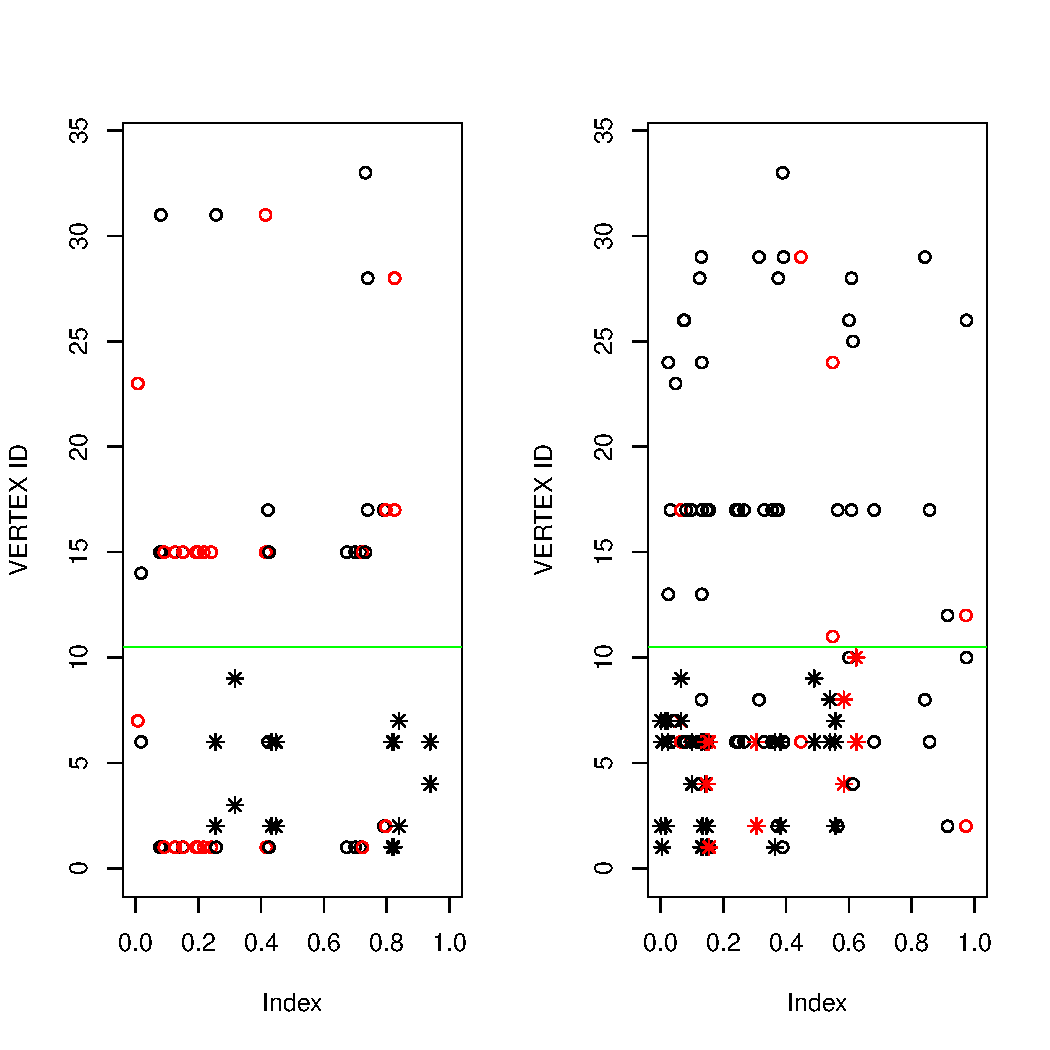
\includegraphics[scale=0.50]{myDdata_w38w58.pdf}
\end{center}
\end{figure}
The subset of the data $\mathcal D$ is presented above only for thirty four vertices in the data.  For clarity, we define given a sub-collection $\mathcal V$ of vertices, we let $\mathcal D(V)$ denote the subsubet of $\mathcal D$, where both the sender and the receiver are from $\mathcal V$. The method in [GC] suggests that the ten vertices out of 184 vertices form a coherent social/communication group.   We aim to support the claim here.

In the following figures the left hand side is for week 38 and the right hand side is for week 58. 
\begin{figure}
\begin{center}
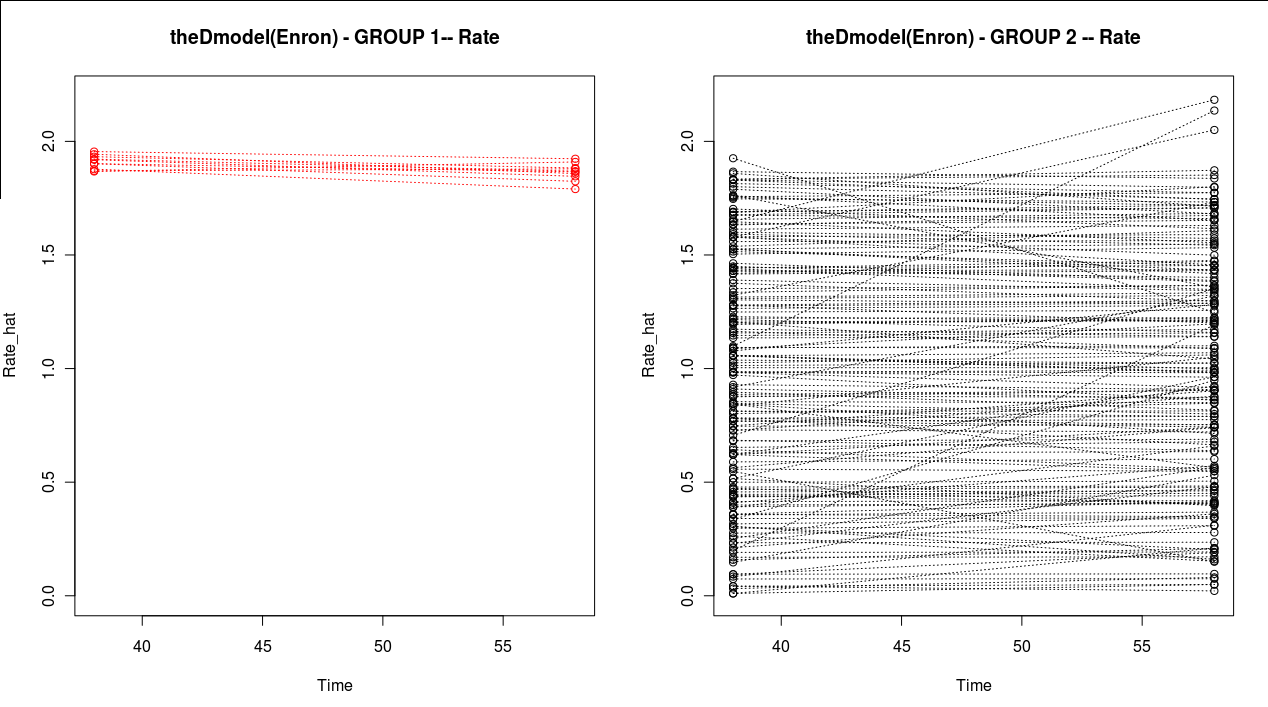
\includegraphics[scale=0.25]{v184_w38vsw58_Rate.png}
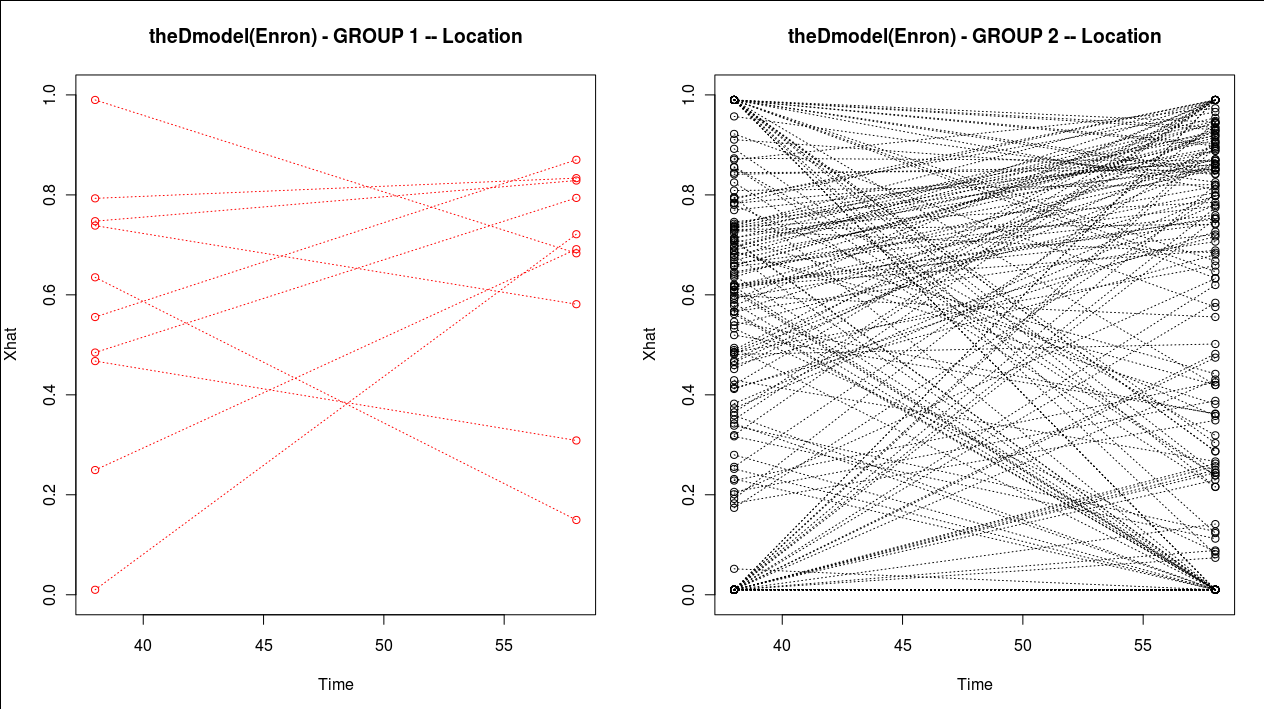
\includegraphics[scale=0.25]{v184_w38vsw58_Location.png}
\end{center}
\end{figure}





\end{document}
